\section{Introduction}
There exists a large number of simulation packages which allow the convenient creation of System Dynamics simulations by straight-forward visual diagram creation. One simply creates stocks and flows, connects them, specifies the flow-rates and initial parameters and then runs them. An example for such a visual diagram creation in the simulation package AnyLogic can be seen in Figure \ref{fig:sir_stockflow_diagram}.

\begin{figure}
	\centering
	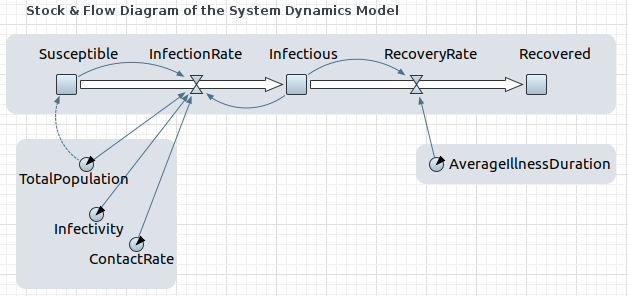
\includegraphics[width=.4\textwidth, angle=0]{./fig/SIR_SD_STOCKFLOW_DIAGRAMM.png}
	\caption{Visual System Dynamics Diagram in AnyLogic Personal Learning Edition 8.3.1.}
	\label{fig:sir_stockflow_diagram}
\end{figure}

The aim of this paper is to look into how System Dynamics can be implemented in raw code without the use of a simulation package. Our language of choice is Haskell because TODO.

We use the well known SIR model \cite{kermack_contribution_1927} from epidemiology to demonstrate our approach.

The contribution of the paper is the demonstration of how a correct-by-construction System Dynamics simulation can be implemented using Haskell.